\section{Product perspective}
\subsection{Scenarios}

\subsubsection{ Educator creates a tournament }
The educator A wants to create a new tournament, he enters the KCB with his educator credentials, once on the homepage he can go into the section "create a new tournament" and fill out a form asking name, main context, enrolment deadline. Now he is able to create or add battles for it.

\subsubsection{ Educator creates a Battle for a specific tournament}
The educator B, owner of a tournament 1, wants to create a battle for his tournament. He enters the KCB with his educator credentials, he goes into the tournament section, selects the tournament 1, and he can go into the "create new battle" section. In this section he can fill a form with the data of the battle such as the battle name, the code template, the registration deadline, the final submission deadline, the quality aspects of that battle which are used for the scoring and sets the minimum and the maximum number of students per group that can participate in that battle. The educator defines a set of categories such that :

    -functional aspects: measured in terms of the number of test cases that pass out of all test cases; 
    
    -timeliness, measured in terms of the time passed between the registration deadline and the last commit;
    
    -quality level:extracted through static analysis tools that consider multiple aspects such as reliability, security, and so on.

The educator gives to each category a  weight.    

\subsubsection{Owner gives permission to another educator to add a Battle}
The owner, the educator C, goes to the section dedicated to the tournament and gives permission to other educators to create new battles by pressing a button to share the control of a tournament. As a consequence the system shows the educator a bar that let him to search other educators. The educator can choose the other educators so an educator D can create a new battle, filling the same form described in the previous scenario. 

\subsubsection{ A student creates a team and invites others to join}
Student E, who already has a profile on the platform, will receive a notification as soon as a new tournament is created. Once he is on the platform, he can read the main information about the tournament and decide whether to join it by the given deadline.
He can create a team for a battle inviting other students, respecting the minimum number of student imposed for the battle of that tournament. To do that, the student will share with his teammate a link to join the battle.

\subsubsection{ A member of the team enrols in a battle}
Student F wants to join her friend on a team for a battle, she received an email with the link that allows her to participate in the battle. She opens the link and thanks to her platform credentials she can join his friend's team.
She knows that students cannot join more than one team for a specific battle.
Once on the platform, she will be able to see in the tournament section the tournament she has registered in and the team she just joined.

\subsubsection{The battle begins}
As soon as the deadline expires, the platform creates the GitHub repository and for each team enrolled sends a notification with a link containing the code kata of the battle. The student G, who has enrolled into this battle, after receiving the notification opens the link and use his credentials to access the source code provided.

\subsubsection{A member of the team pushes and commit to the kata repository}
Student H who is enrolled in a battle, finishes to code the kata with his teammates and wants to submit it. In order to do that, he should fork the GitHub repository of the kata and set up the automated workflow if no one has done it before.
Thanks to this action the platform will be triggered every time any of the team members pushes a new commit into the main branch of the repository. Afterwards he pushes and commits being able to see the new results on the platform.

\subsubsection{ The battle ends}
At the end of the battle the platform updates the tournament score of every student enrolled, by recomputing the scores considering all battles belonging to that tournament.


\subsubsection{ Educator manually evaluates the code provided by students}
Educator L who contributed to the creation of the tournament has the possibility to manually evaluate the work done by a team at the end of each battle. In order to do that, he can access the platform with his credentials, and go to the tournament section, then open the battle information and go through the sources produced by each team. Afterwards, he will assign a score that will be considered by the platform when the final ranking is computed.

\subsubsection{ Users see the final rank of the tournament}
Educator M closes the tournament thanks to the button 'end tournament' in the tournament section of the KCB platform. As a consequence of that, the platform elaborate the final rank for each student involved to that tournament and finally notify them about it. 
Student N who participated to the tournament and received the notification via e-mail can consult the final ranking by selecting the tournament into the 'tournament section' of the platform.

\subsubsection{ Users can see current rank}
User J (an educators or a student) involved in a battle is allowed to see the evolving rank during the battles. They can consult the ranking into the dedicated section of the battle and compare students' performances.
Every user has the possibility to consult the "ongoing tournament section"in which it is possible to see the list of the ranking for each tournament in progress. 

\subsubsection{Student receives a badge}
When a tournament ends the platform assign the badges to the students that satisfied the requirements to obtain them.
As previously mentioned, the criteria for assigning the badge are defined by the educators during the creation of the tournament.
Any user subscribed to the platform can view the badges collected by any student so far. So student P who want to see the total number of badges can access the platform with his credentials and see them on his profile. He can also view the badges collected by his friend Student Q, in order to do that he can look for student Q profile and check the number of badges his friend has collected so far.
\pagebreak



\subsection{ Domain class diagram}
\begin{figure}[h!]
\centering
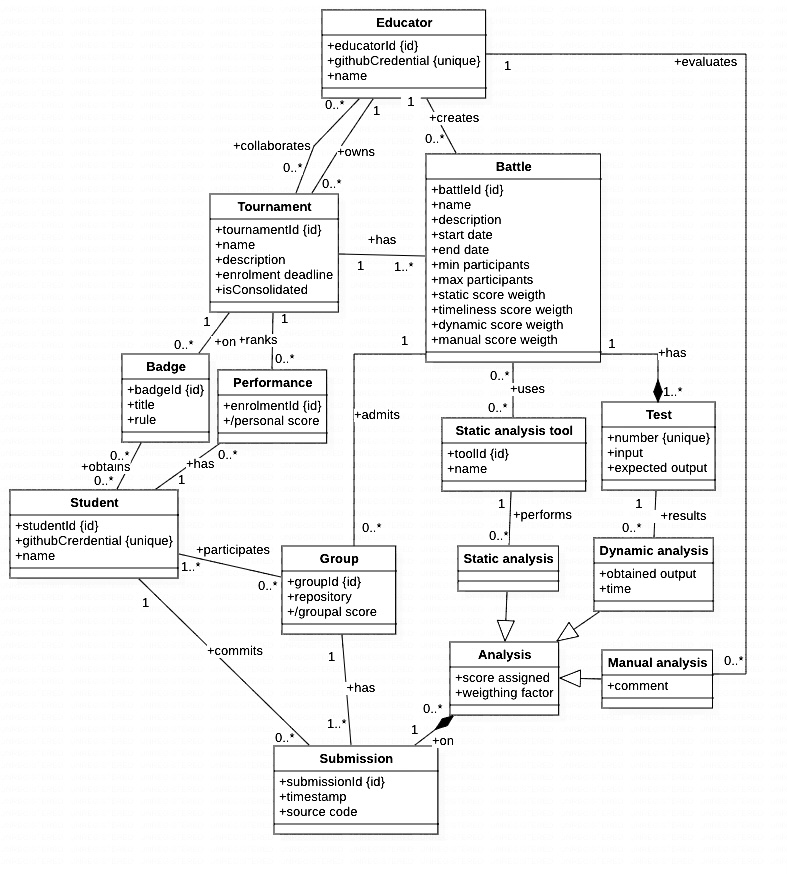
\includegraphics[width=\textwidth]{Images/dcd.jpg}
\caption{Domain class diagram}
\label{dcd}
\end{figure}

In Figure \labelcref{dcd} you can find the domain class diagram. Despite both educators and students being user, we represent  them separately in the diagram.  As it was mentioned educators can own a tournament or simply collaborate in other's. The tournament has only one owner but can have many collaborators. 

Tournaments consists of many battles which are created for that specific tournament. Then for the scoring it is necessary that the battle has the weights for each type of analysis (static, timeliness, dynamic and manual). As well as the static tools to be used and the tests to evaluate that specific battle.

Afterwards, with all this different types of analysis it will be possible to perform the whole analysis on a particular submission. All the analysis regardless of the type will contribute on the score of the submission similarly. Note that Timeliness is not represented like the other analysis because the submission already contains the timestamp which is sufficient for that purpose. Although it could not be represented in the diagram, the weighing factor of the analysis, the tools used and the executed tests have to be consistent with the ones defined in the battle that submission corresponds. In the same way, the educator who evaluates should be the one responsible of that battle.

In order to participate in a battle students have to make a group this is only correspond to one battle and contains the Github repository from which submissions will be collected each time the source code is modified and committed. Then the score of the group will be taken from the best submission. In the diagram we could not represent that students can only participate only once in a battle, however this is relevant.

Finally, the tournament will have many badges which then will be assigned to the students following the rule criteria. This was not represented neither that students can only have badges for tournaments in which the took part.

\subsection{State diagrams}
In this subsection there is a discussion of the state charts diagram the ones for the management of the battles and the tournaments.Both of them are necessary for having a better understanding of how battles and tournaments works.

\textbf{Tournament management}

\begin{figure}[h!]
\centering
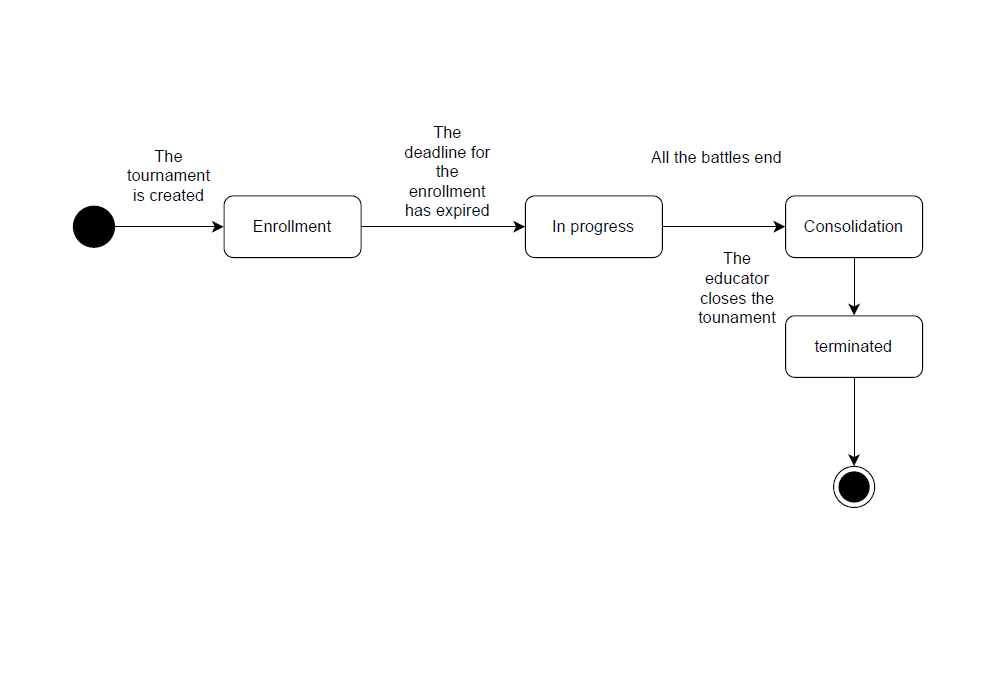
\includegraphics[width=12cm]{Images/tournament.png}
\caption{Tournament state charts}
\label{dcd}
\end{figure}



In this state charts diagram is explained how a tournament works and the different states that it has.In the\textit{ Enrollment} state the students enroll in the tournament and is the very first state after the educator has created the tournament.
The \textit{In progress} state represents the state in which the deadline for the enrollment has expired and the tournaments begins so the battle are going to be attended.The second-last state is \textit{Consolidation} in which all the battles are ended.The last state is the \textit{Terminated} in which the educator ends the tournament.

\textbf{Battle management}

\begin{figure}[h!]
\centering
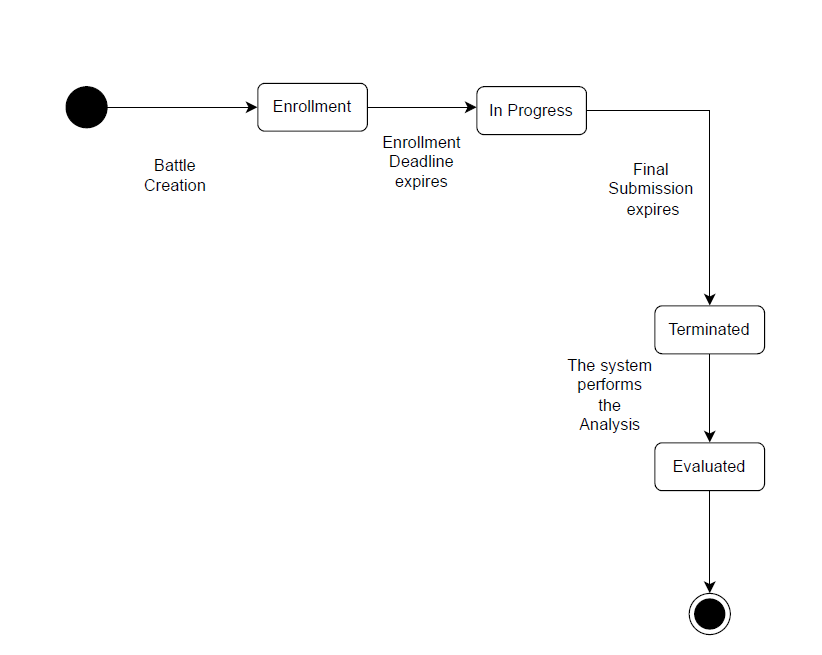
\includegraphics[width=12cm]{Images/startBattle.png}
\caption{Battle state charts}
\label{dcd}
\end{figure}

In this state chart diagram is explained how a battle works and the different states that it has. In the\textit{ Enrolment} state the students enrol in the battle and it is the very first state after the educator has created the battle.
The \textit{In progress} state represents the state in which the deadline for the enrollment has expired and the tournaments begins so the battle is going to be attended.The second-last state is \textit{Terminated} in which the battle is ended.The last state is  \textit{Evaluated} in which the system analysis has been performed and an evaluation has given either by the system or the educator.

\section{Product functions}
\subsubsection{Sign up and log in}
Sign-up is available to all users who want to subscribe to the platform. When a new user opens the platform, he will press the button 'Sign-in'. The user will then be redirected to GitHub \footnote{We decide to require users to use their GitHub account to sign. We already required students to have one to participate in the tournament, and this simplifies the process of checking who submitted the code, as each user is linked to one GitHub account. Also this decision could in the future allow us to seamlessly add more functionalities,  such as creating the web-hooks or forking the kata automatically and others that will ease the work of educators as well} where they are required to log in or create an account in order to link their GitHub account with our platform. Once this operation is completed, the platform will ask the user extra information, such as a username, so that the platform can create the user profile. Once the profile is created, the system allows the user to log into the platform for the first time using his GitHub account.\cite{githubOAuth}

\subsubsection{Tournament and battles management}
This function is only available to the educator. Their role is to create a tournament which consist of several battles that are related by the same topic. The first creator of the tournament allows his colleagues to contribute to the creation of the tournament by giving them the permission to add, modify, or delete battles for that tournament.
The teacher should provide the students with the necessary materials to do the kata and should also define the minimum and maximum number of students allowed for the battle. Finally, he should specify the deadlines for both registration to the battle and final submission of the code.

\subsubsection{Teams creation}
This function is available to all student who wants to create a team and join a battle. Once the team leader has signed up for the battle, it has the possibility to share an invitation link with other registered students. The students who received the invitation link can join the team-leader and subscribe to the battle.

\subsubsection{Scoring and ranking}
This function is available to any educator who wants to score and rank a group of students for their coding abilities. after a battle the educator has the possibility to manually evaluate the team that has uploaded the code based on some criteria.

\subsubsection{Badges}
This function allows educator to creates badges which are a reward for students achievements. The criteria to assign the badges are decided by the educator during the tournament creation.
Thanks to this function, every user can view the badges collected by each student by visiting their profile.

\subsubsection{Tournament and battles participation}
The students that are registered to the platform will receive a notification. Therefore, they can subscribe to the tournament after registering and will be informed of every incoming battle.
For what concerns each battle the students can form a team by using the platform they should create a repository on github if they do not create it, the platform will create it after the registration deadline.Then, the students have to fork the repository and they can start working on their project creating a workflow on github.Every push triggers the platform that starts doing the tests

\subsubsection{Tournament and battles consolidation}
This function allows the system to evaluate the code pushed by each team and assign it a score. This score is updated every time a new push is made into the repository.
When the battle ends, the educator who created the battle has the possibility to manually evaluate the code done by the teams for that battle by going through the sources implemented by the students. This phase is called consolidation because right after the manual evaluation the final score of the battle is calculated and all students who participate to it are notified about the ranking.

\section{User Characteristics}
There are mainly two types of user that interact with the platform: student and educator.

\subsection{Student}
The student  is able to register and login to the platform and is also allowed to participate to a tournament after the tournament if his performances will be good he will receive a badge based on the rules that he fulfilled

\subsection{Educator}
The educator is a user who can create a tournament and the battle inside of it.This type of user can also evaluate students after the battle and create a badge that will be assigned to students who had the best performances.



\pagebreak
\section{Assumptions, dependencies and constraints}

\subsection{Regulatory policies}
The CKB application asks for the GitHub account information. GitHub will not be used for commercial purposes. Personal information will be processed in compliance with the GPDR.

\subsection{Domain Assumptions}
The following assumptions are made for the domain. They are properties or conditions that the system will take for granted.They must be checked to ensure a correct platform behaviour
\begin{enumerate}[label={[D\arabic*]}]

    \item User must have a reliable internet connection
    \item User personal information must be correct
    \item Educators properly insert information about a tournament
    \item The Github interaction it's reliable( the user is able to pull and push the code without losing its data)
    \item Notifications to the user must arrive as soon as the final rank is available
    \item The Educator properly insert an evaluation manually when it's requested
    \item The educator correctly adds information about a new badge such as new rules or badge name
    
\end{enumerate}